\documentclass[aps,prb,reprint,twocolumns,superscriptaddress,nofootinbib]{revtex4-2}
\usepackage[utf8]{inputenc}
\usepackage{amsmath}
\usepackage{amssymb}
\usepackage{txfonts}
\usepackage[hidelinks]{hyperref}
\usepackage{tikz}
\usepackage{hyperref}
\usepackage{color}
\hypersetup{colorlinks=true}
\usepackage{graphicx}
\graphicspath{{figures}}
\usepackage{bm}

\usepackage{chemformula}
\usepackage[capitalise]{cleveref}
\usepackage{siunitx}
\newcommand{\hc}{\text{h.c.}}
\newcommand{\ii}{\mathrm{i}}
\newcommand{\pg}[1]{\textcolor{red}{PG: #1}}
\DeclareMathOperator{\sign}{sign}
\DeclareMathOperator{\Imm}{Im}
\DeclareMathOperator{\Ree}{Re}

\newcommand{\xx}{\hat{\bm{x}}}
\newcommand{\yy}{\hat{\bm{y}}}
\newcommand{\mdos}{\tilde{m}}
\newcommand{\kF}{k_{F}}
\renewcommand{\thefigure}{S\arabic{figure}}
\renewcommand{\theequation}{S\arabic{equation}}
\renewcommand{\thetable}{S\Roman{table}}
\renewcommand{\thesection}{\Roman{section}}
\newcommand{\subfigref}[2]{Fig.~\hyperref[#1]{\ref*{#1}#2}}

\newcommand{\FermileveltwoD}{\SI{0.5}{eV}}
\newcommand{\twoDratio}{0.84}
\newcommand{\criticalangle}{\SI{39.9}{\degree}}
\newcommand{\Fermilevel}{\SI{0.5}{eV}}
\newcommand{\mstar}{1.25}
\newcommand{\mzero}{0.4}
\newcommand{\splitting}{\SI{0.6}{eV}}
\newcommand{\muB}{0.025}
\newcommand{\muBShift}{\SI{1.5}{\mu eV}}
\newcommand{\demonenergy}{\SI{2.8}{meV}}
\newcommand{\muBShiftrelative}{0.1}
\newcommand{\muBmax}{0.1}

\usepackage{zref-xr}
\zxrsetup{toltxlabel}

\zexternaldocument*{prl_main}

\begin{document}
	\title{Supplementary Material: Spin demons in $d$-wave altermagnets}
	\date{\today}
	
	\author{Pieter M. Gunnink}
	\email{pgunnink@uni-mainz.de}
	\author{Jairo Sinova}
	\author{Alexander Mook}
	\address{Johannes Gutenberg University Mainz, Staudingerweg 7, Mainz 55128, Germany}
	\begin{abstract}
		
	\end{abstract}
	
	\maketitle
	
	
	
	\section{Three-dimensional planar $d$-wave altermagnet}
	We consider a three-dimensional $d$-wave altermagnet, where the low-energy electron dispersion of spin $\sigma$ can be written as \cite{smejkalEmergingResearchLandscape2022,smejkalAnomalousHallAntiferromagnets2022}
	\begin{align}
		\epsilon_{\bm k}^\sigma &= \frac{\hbar k^2}{2m_0} + \sigma \frac{\hbar k_x^2}{2m_*} - \sigma \frac{\hbar k_y^2}{2m_*} \\
		&=\frac{\hbar k_x^2}{2m_x^\sigma}+ \frac{\hbar k_y^2}{2m_y^\sigma} +\frac{\hbar k_z^2}{2m_z}
	\end{align}
	where $m_0$ is the effective (isotropic) mass and $m_*$ is the altermagnetic splitting mass, and $k=|\bm k|$. We stress that we have defined the altermagnetic splitting mass such that $m_0<m_*$. Furthermore, we have defined for convenience
	\begin{align}
		m_x^\sigma &\equiv m_0 m_* / (m_*+\sigma m_0) \label{eq:my} \\
		m_y^\sigma&\equiv m_0 m_* / (m_*-\sigma m_0)  \label{eq:mx}\\ 
		m_z&\equiv m_0.
	\end{align} 
	Within this orientation, the altermagnetic spin-split plane is the $xy$-plane, and spin splitting is maximal for $\bm k \parallel \xx$ and $\bm k \parallel \yy$, while vanishing along the diagonals.
	
	We show the dispersion in \cref{fig:dispersion} along the two maximal spin splitting directions, for the parameters as used in the main text: $m_0=\mzero m_e$, $m_*=\mstar m_0$ and $E_F=\Fermilevel$, where $m_e$ is the electron mass.
	\begin{figure}
		\centering
		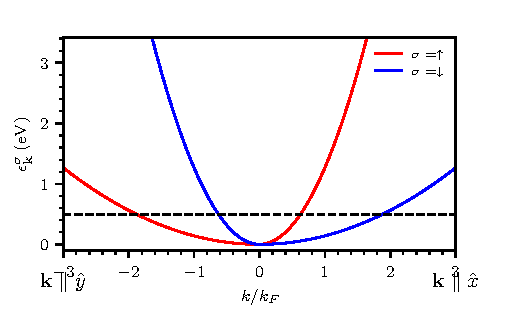
\includegraphics{dispersion}
		\caption{Low-energy electron dispersion of spin $\sigma$, along the two maximal spin splitting directions. Here, $k$ is given in units of the spin-independent Fermi wave vector, as defined in \cref{eq:kF}. The Fermi level is indicated with the horizontal dashed line. Additionally, $m_0=\mzero m_e$, $m_*=\mstar m_0$ and $E_F=\Fermilevel$, where $m_e$ is the electron mass. \label{fig:dispersion}} 
	\end{figure}
	
	\section{Spin resolved response functions}
	The spin resolved response function of an altermagnet is given in the random phase approximation (RPA) by \cite{giulianiQuantumTheoryElectron2005}
	\begin{equation}
		\begin{pmatrix}
			\chi_{\uparrow\uparrow} & \chi_{\uparrow\downarrow} \\ 
			\chi_{\downarrow\uparrow} & \chi_{\downarrow\downarrow}
		\end{pmatrix}^{-1} = \begin{pmatrix}
			\chi_\uparrow^{(0)} & 0 \\
			0 & \chi_\downarrow^{(0)}
		\end{pmatrix}
		- v_q \begin{pmatrix}
			1 & 1 \\ 1 & 1 
		\end{pmatrix} \label{eq:chi-rpa}
	\end{equation}
	where $\chi_\sigma^{(0)}$ is the spin-resolved non-interacting density-density response function and $v_q=e^2 / (\epsilon q^2)$ is the three-dimensional Fourier transform of the Coulomb interaction, with $q=|\bm q|$. The spin-resolved non-interacting density-density response function can be found by evaluating the Lindhard function
	\begin{equation}
		\chi_\sigma^{(0)}(\omega,\bm q) \equiv \frac{1}{V} \sum_{\bm k} \frac{n_{\bm k}^\sigma - n_{\bm k-\bm q}^\sigma}{\hbar\omega + \epsilon_{\bm k}^\sigma - \epsilon_{\bm k-\bm q}^\sigma},
	\end{equation}
	where $V$ is the volume. The Lindhard function can be evaluated as in the isotropic result \cite{giulianiQuantumTheoryElectron2005}, by rescaling $q_\lambda\rightarrow \sqrt{\mdos/m_\lambda^\sigma} q$ and $m\rightarrow \mdos$ \cite{ahnAnisotropicFermionicQuasiparticles2021}, for $\lambda\in\{x,y,z\}$, 	 where
	\begin{align}
		\mdos&\equiv \sqrt[3]{m^\sigma_xm^\sigma_ym_z} \nonumber\\
		&=m_0\sqrt[3]{m_*/(m_*^2-m_0^2)}.
	\end{align}
	For convenience, we define 
	\begin{align}
		\kF&\equiv\sqrt{2\mdos E_F}/\hbar, \label{eq:kF} \\
		v_F&\equiv \hbar k_F/\mdos,
	\end{align}
	as the spin-independent Fermi wave vector and velocity respectively. We stress that $\kF$ does not correspond to the actual Fermi wave vector, which is spin and $\bm k$ dependent.
	
	
	We focus in this work on wave vectors $\bm q$ lying in the altermagnetic spin-split plane, and thus parametrize
	\begin{equation}
		\bm q = q\cos\theta\,\hat{\bm x} + q\sin\theta\,\hat{\bm y}.
	\end{equation}
	We can  rewrite the above rescaling as $q\rightarrow \eta_\sigma q$, where
	\begin{equation}
		\eta_{\sigma}(\theta) \equiv \sqrt{\mdos m_0\left( 1+\sigma \frac{m_0}{m_*}\cos2\theta\right)} \label{eq:sigma},
	\end{equation}
	is the projected spin splitting for spin species $\sigma$ at an angle $\theta$. In what follows, we suppress the $\theta$ label.
	
	We obtain
	\begin{multline}
		-\frac{\Ree[\chi_\sigma^{(0)}]}{N_0} = \frac{1}{2}-\frac{1-\nu_{-\sigma}^2}{4\eta_\sigma \bar q}\log\left|\frac{\nu_{-\sigma}+1}{\nu_{-\sigma}-1}\right|\\+\frac{1-\nu_{+\sigma}^2}{4\eta_\sigma \bar q}\log\left|\frac{\nu_{+\sigma}+1}{\nu_{+\sigma}-1}\right| \label{eq:rechi0}
	\end{multline}
	and
	\begin{multline}
		-\frac{\Imm[\chi_\sigma^{(0)}]}{N_0} = \frac{\pi }{4\eta_\sigma \bar q}\Bigr[\Theta(1-\nu_{-\sigma}^2)(1-\nu_{-\sigma}^2)\\
		-\Theta(1-\nu_{+\sigma}^2)(1-\nu_{+\sigma}^2)\Bigr], \label{eq:imchi0}
	\end{multline}
	where 
	\begin{align}
		\nu_{\pm\sigma} &\equiv \frac{\omega}{\eta_\sigma qv_F} \pm \frac{1}{2}\eta_\sigma \bar q, \\
		\bar q &\equiv \frac{q}{\kF},	\end{align}
	and 
	\begin{equation}
		N_0 \equiv \frac{\mdos \kF}{2\pi^2\hbar^2}
	\end{equation}
	is the spin-independent density of states at the Fermi level. Finally, $\theta(x)$ is the Heaviside step function.
	
	Additionally, the edges of the spin-resolved particle-hole continua are given by 
	\begin{equation}
		\max[0,\omega_{-\sigma}] \leq |\omega| \leq \omega_{+\sigma} \label{eq:boundaries}
	\end{equation}
	where 
	\begin{equation}
		\omega_{\pm\sigma} = \frac{\hbar \eta_\sigma^2q^2}{2\mdos} \pm \eta_\sigma v_F q.\label{eq:omegapm}
	\end{equation}
	
	
	Solving \cref{eq:chi-rpa} for $\chi_{\sigma\sigma'}(\bm q,\omega)$, we find the density-density, spin-spin and density-spin response functions, respectively given by
	\begin{align}
		\chi_{nn}(\bm q,\omega) &= \frac{S(\bm q,\omega)}{\epsilon(\bm q,\omega)}, \label{eq:chinn}\\
		\chi_{S_zS_z}(\bm q,\omega)&=\frac{S(\bm q,\omega)-4v_q(\bm q,\omega)P(\bm q,\omega)}{\epsilon(\bm q,\omega)} ,\label{eq:chiSzSz}\\
		\chi_{nS_z}(\bm q,\omega)&=\frac{D(\bm q,\omega)}{\epsilon(\bm q,\omega)} ,\label{eq:chinSz}
	\end{align}
	where 
	\begin{equation}
		\epsilon(\bm q,\omega) \equiv 1 - v_qS(\bm q,\omega) \label{eq:epsilon}
	\end{equation}
	is the complex longitudinal dielectric function and $S(\bm q,\omega)\equiv\sum_\sigma \chi_\sigma (\bm q,\omega)$, $D(\bm q,\omega)\equiv\chi_\uparrow (\bm q,\omega)-\chi_\downarrow (\bm q,\omega)$ and $P(\bm q,\omega)\equiv\Pi_\sigma \chi_\sigma (\bm q,\omega)$. 
	
	Collective modes emerge as the poles of the response functions. Since $S(\bm q,\omega)$, $D(\bm q,\omega)$ and $P(\bm q,\omega)$ are smooth functions of momentum and frequency, the poles are determined by the zeros of the longitudinal dielectric function, 
	\begin{equation}
		\epsilon(\bm q,\omega) = 0. \label{eq:poles}
	\end{equation}
	\section{Density-density and density-spin response functions} 
	In the main text we have focused on $\chi_{S_zS_z}(\bm q,\omega)$. Here, we discuss the two other response functions, $\chi_{nn}(\bm q,\omega),\ \chi_{nS_z}(\bm q,\omega)$.	
	We show in \cref{fig:all-chis} all three response functions at a fixed $q=0.05\kF$, where we have rescaled $\chi_{nn}(\bm q,\omega),\ \chi_{nS_z}(\bm q,\omega)$ to allow for a direct comparison. We remind the reader that a zero of the dielectric function, \cref{eq:epsilon}, will result in a collective mode in all three response function---but its actual experimental response is determined by the numerator of the relevant response function, \cref{eq:chinn,eq:chiSzSz,eq:chinSz}. 
	
	We first observe that there is no well-defined quasiparticle peak in $\Imm[\chi_{nn}(\bm q,\omega)]$, in contrast to $\Imm[\chi_{nS_z}(\bm q,\omega)]$ and $\Imm[\chi_{S_zS_z}(\bm q,\omega)]$. However, the response of $\Imm[\chi_{nS_z}(\bm q,\omega)]$ is much weaker than of $\Imm[\chi_{S_zS_z}(\bm q,\omega)]$ (note the rescaling by a factor of $10^4$). 	
	The conventional charge plasmon would however appear in $\chi_{nn}(\bm q,\omega)$, but is gapped and thus lives at much higher frequencies in a three-dimensional metal.
	
	We therefore focus on $\chi_{nS_z}(\bm q,\omega)$, and show $\Imm[\chi_{nS_z}(\bm q,\omega)]$ as a function of wave vector $\bm q$ and frequency $\omega$ in \cref{fig:chi-nSz}. This is the equivalent of \cref{fig:alongx} in the main text. This demonstrates that $\chi_{nS_z}(\bm q,\omega) $ can also serve as a probe of the spin demon, although its signal is much weaker (a factor of $10^4$) than the response in the $\chi_{S_zS_z}(\bm q,\omega)$ channel.
	\begin{figure}
		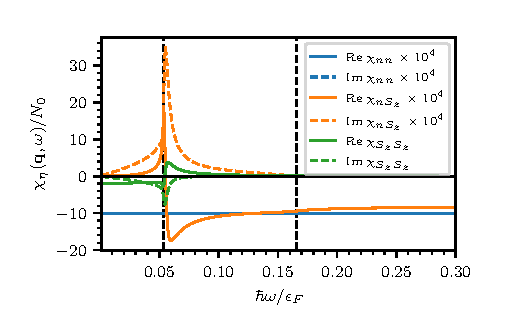
\includegraphics{linecut-chi_nn}
		\caption{The three fundamental response functions, $\chi_{nn}, \chi_{nS_z}$ and $\chi_{S_zS_z}$, where we have rescaled $\chi_{nn}, \chi_{nS_z}$ to facilitate a direction comparison. Here we have set $q=0.05\kF$. Note that $\Imm[\chi_{nS_z}]>0$ does not violate causality, since $\Imm[\chi_{\sigma\sigma'}]<0$ for all $\sigma,\sigma'\in\lbrace\uparrow,\downarrow\rbrace$. \label{fig:all-chis} }
	\end{figure}
	
	\begin{figure}
		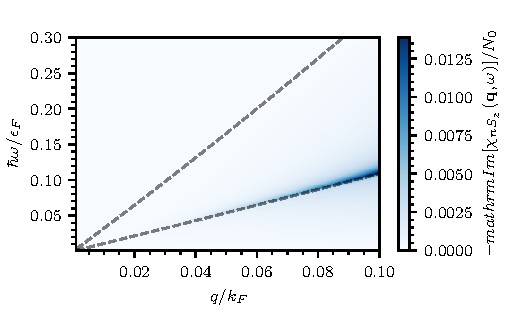
\includegraphics{nSz_3D}
		\caption{$\Imm[\chi_{nS_z}]$ as a function of wave vector $\bm q$ and frequency $\omega$, showing that $\chi_{nS_z}$ could also be used to detect the spin demon---but note that the response is a factor of $10^4$ weaker than in $\Imm[\chi_{S_zS_z}]$. The equivalent of \cref{fig:alongx} in the main text. \label{fig:chi-nSz}}
	\end{figure}
	
	
	
	\section{Spin demon with finite out-of-plane wave vector}
	\begin{figure*}
		\begin{tikzpicture}
			\node at (-0.5\columnwidth,0) {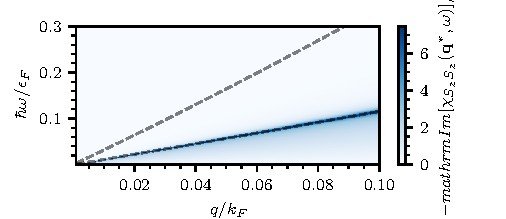
\includegraphics[width=\columnwidth]{SzSz_3D_theta_10}};
			\node at (0.5\columnwidth,0) {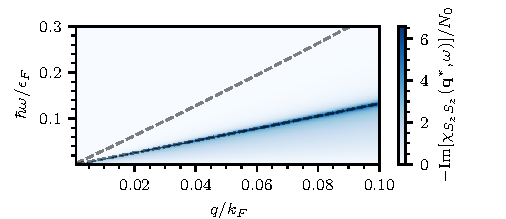
\includegraphics[width=\columnwidth]{SzSz_3D_theta_20}};
			\node at (-0.5\columnwidth,-4) {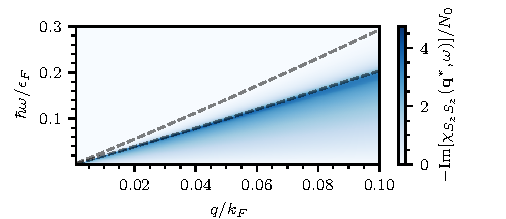
\includegraphics[width=\columnwidth]{SzSz_3D_theta_50}};
			\node at (0.5\columnwidth,-4) {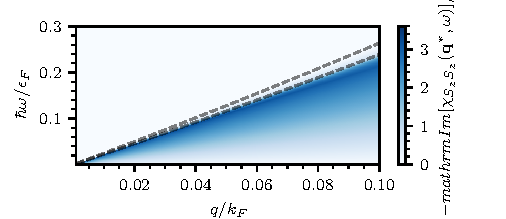
\includegraphics[width=\columnwidth]{SzSz_3D_theta_70}};
			\node at (-0.5\columnwidth,1.8) {$\psi=\SI{10}{\degree}$};
			\node at (0.5\columnwidth,1.8) {$\psi=\SI{20}{\degree}$};
			\node at (-0.5\columnwidth,-2.3) {$\psi=\SI{50}{\degree}$};
			\node at (0.5\columnwidth,-2.3) {$\psi=\SI{70}{\degree}$};
		\end{tikzpicture}
		\caption{The spin-spin response function $\chi_{S_zS_z}(\bm q^*,\omega)$, where $\bm q^*=q\ (\cos\psi,0,\sin\psi)$, such that the spin demon gains a finite out-of-plane wave vector component. The dashed lines indicate the edges of the spin-resolved particle-hole continua. \label{fig:oop}}
	\end{figure*}
	
	Here, we consider the effect of a finite out-of-plane wave vector on the quality factor of the spin demon. We parametrize $\bm q^* = q\ (\cos\psi,0,\sin\psi)$, and show the resulting spin-spin response function in \cref{fig:oop}, for increasing angles $\psi$. We first observe that for small angles $\psi$, there is little change to the spin demon dispersion (compare $\psi=\SI{10}{\degree},\SI{20}{\degree}$ with \subfigref{fig:alongx}{(b)} in the main text). The quality factor does however decrease, which we also expect, since the spin splitting and thus the separation of the particle-hole continua decreases for $q_z\neq0$. In particular, for high angles $\psi$, the spin demon is washed out, and is no longer well defined. Importantly, this effect becomes only apparent for higher angles $\psi$, and we thus expect that the spin demon is well defined even if the experimental probe is not perfectly aligned with the altermagnetic spin-split plane.
	
	
	
	\section{Details of numerics}
	\label{sec:numerics}
	The dielectric function, \cref{eq:epsilon}, can be evaluated exactly using the analytical expressions \cref{eq:rechi0,eq:imchi0}. We  numerically obtain the zeros of $\epsilon(\bm q,\omega)$ as a function of $\omega$ using the Roots.jl package \cite{Roots.jl}.
	
	
	To determine the corresponding quality factor, we perform a numerical derivative of the dielectric function at this pole by central difference as
	\begin{equation}
		\frac{\partial\epsilon}{\partial\omega}\big|_{\omega=\omega_{d}} \approx \frac{\epsilon|_{\omega=\omega_{d}+\delta_\omega}-\epsilon|_{\omega=\omega_{d}-\delta_\omega}}{2\delta\omega},
	\end{equation}
	where we set $\hbar\delta_\omega=10^{-4}\epsilon_F$ and $\omega_d$ is the numerically obtained pole of $\epsilon(\bm q,\omega)$ which corresponds to the spin demon (i.e., the numbered with a 2 in \subfigref{fig:alongx}{(a)} in the main text). We can then directly evaluate the damping rate $\gamma=\Imm[\epsilon]/\partial_\omega\Ree[\epsilon]$.
	
	To determine the magnetic moment, we numerically evaluate
	\begin{equation}
		\mu = -\hbar\frac{\partial\Delta}{\partial B} \frac{\omega_d|_{+\Delta}-\omega_d|_{-\Delta}}{2\Delta},
	\end{equation}
	where $\omega_d|_{\pm\Delta}$ is the numerically obtained spin demon pole with a magnetic field $\pm\Delta(B)$, as defined in \cref{eq:Delta}. We refer the reader to  \cref{sec:magnetic-moment} for a detailed derivation of the magnetic moment.
	
	
	
	\section{Analytical solution of spin demon dispersion}
	We now turn to solving \cref{eq:poles} for an (approximate) solution to the dispersion of the spin demon. 	
	We first consider the case where $\bm q\parallel \xx$. Then, spin down is the minority spin species, and from numerics (\cref{fig:alongx} in the main text), we know the spin demon to live close to the edge of the minority spin particle-hole continuum.
	
	Following the approach by \textcite{santoroAcousticPlasmonsConducting1988}, we therefore make the ansatz\footnote{This ansatz is motivated by the structure of $\chi_\sigma(\bm q,\omega)$.}  
	\begin{equation}
		\omega_d = v_s \eta_{\downarrow}(\theta)q. \label{eq:ansatz}
	\end{equation}
	Here $v_s$ is the spin demon velocity, which is to be determined.
	
	
	Additionally, we require that the spin demon lives in the pseudogap between the boundaries of the spin-down and spin-up particle hole continuum. These bounds are given by [see \cref{eq:boundaries,eq:omegapm}]
	\begin{equation}
		\omega_{+\sigma} = \frac{\hbar\eta_\sigma^2(\theta) q^2}{2\mdos} + v_F  \eta_\sigma(\theta) q. \label{eq:particle-hole-bounds}
	\end{equation}
	Inserting our ansatz [\cref{eq:ansatz}] into \cref{eq:particle-hole-bounds}, we find that we require that $\tilde v_s < \delta_q^{-1}$, where we have defined
	\begin{align}
		\delta_q(\theta)&\equiv \frac{\eta_\downarrow(\theta)}{\eta_\uparrow(\theta)} \\
		\tilde v_s&\equiv  \frac{v_s}{v_F}.
	\end{align}
	
	As was discussed before, collective modes appear as zeros of the longitudinal dielectric function [\cref{eq:epsilon}]. We therefore insert our ansatz in \cref{eq:epsilon}, and solve for $v_s$. Since $v_q\propto q^{-2}$, we next expand  $\chi_\sigma^{(0)}(\bm q,\omega_d)$ up to second order in $\tilde q$.
	
	Since the spin demon is always located far away from the edge of spin-up particle-hole continuum , the real part of the spin-up particle-hole continuum is approximately constant, $\chi_\uparrow^{(0)}(\bm q,\omega)\approx-N_0$ \cite{giulianiQuantumTheoryElectron2005}.
	%    given by the small $\bar q$ limit of  $\chi_\uparrow^{(0)}$, which is \cite{giulianiQuantumTheoryElectron2005}
	%    \begin{equation}
		%     \chi_\uparrow^{(0)}(\bm q,\omega)=-N_0\left(1-\frac{\omega}{v_F \bar q} \log\left[ \frac{\omega/v_F \bar q +1}{\omega/v_F\bar q -1}\right] \right).
		% \end{equation}
	Inserting out ansatz, we find 
	\begin{equation}
		\Ree[\chi_\uparrow^{(0)}](\bm q,\omega_d) \approx -N_0\left(1-\frac{\delta_q(\theta) \tilde v_s}{2}\log\left[\frac{\delta_q(\theta) \tilde v_s+1}{\delta_q(\theta) \tilde v_s-1}\right]\right) + O\left(\bar q^2\right) \label{eq:chiup-expanded}.
	\end{equation} 
	
	
	
	
	Similarly, we now expand $\chi_\downarrow(\bm q,\omega_d)$ in $q$ to obtain\footnote{Note that the spin demon lives outside of the spin-down particle-hole continuum, and thus $\Imm[\chi_\downarrow(\bm q,\omega_d)]$ is strictly zero.}
	\begin{equation}
		\chi_\downarrow(\bm q,\omega_d) = \frac{N_0}{2}\left(4-\tilde v_s\log \left[ \frac{1+\tilde v_s}{\tilde v_s-1} \right]\right) + O\left(\bar q^2\right) \label{eq:chidown-expanded}.
	\end{equation}
	
	Since $v_q^{-1}=O(\bar q^2)$, $\omega_d=v_s\eta_\downarrow(\theta) q$ is a solution to $\epsilon(\bm q,\omega_d)=0$ if
	\begin{equation}
		4-\tilde v_s\log \left[ \frac{1+\tilde v_s}{\tilde v_s-1}\right] - \delta_q \tilde v_s \log \left[ \frac{1+\delta_q\tilde v_s}{\delta_q\tilde v_s-1}\right] = 0. \label{eq:zeros-epsilon-full}
	\end{equation} 
	This equation cannot be solved analytically for $\delta_q\neq0$. However, for $\delta_q=0$ we can perform a Laurent-Taylor expansion around the pole $\tilde v_s=1$ to find 
	\begin{equation}
		4-\log \left[ \frac{1+\tilde v_s}{\tilde v_s-1}\right] + O(\tilde v_s - 1) = 0,
	\end{equation}
	which can be solved to find $\tilde v_s=1+2e^{-4}\approx1.037$. To compare, we also numerically solve \cref{eq:zeros-epsilon-full} for $\delta_q=0$ to find
	\begin{equation}
		\tilde v_s \approx 1.044.
	\end{equation}
	These result thus show that the spin demon lives at a frequency just above the edge of the particle-hole continuum, which is given by $\tilde v_s=1$.   
	%	We first focus on the limit of strong altermagnetic spin splitting, such that $\delta_q\approx0$ for $\bm q\parallel \hat x$. We can then numerically $4-\tilde v_s\log \left[ \frac{1+\tilde v_s}{\tilde v_s-1}\right] =0$ to find two solutions, but only one of these is in the pseudogap, given by $\tilde v_s=1.044$. 
	
	\begin{figure}
		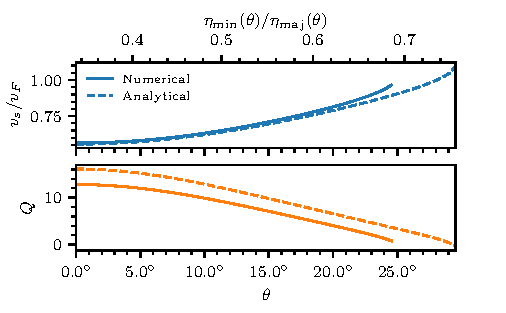
\includegraphics{angles_vs_and_Q_with_eta}
		\caption{The zeros of \cref{eq:zeros-epsilon-full} as a function of $\delta_q$. We only show solutions where the spin demon pole sits inside the pseudogap, i.e., we require $\tilde v_s<\delta_q^{-1}$. Identical to \cref{fig:vs-and-Q} in the main text, except for the top axis, which gives the conversion between the angle $\theta$ and $\delta_q(\theta)=\eta_\downarrow(\theta)/\eta_\uparrow(\theta)$.
			Note that for $\bm q\parallel\xx$ we have that $\eta_{\mathrm{min}}=\eta_{\downarrow}$ and $\eta_{\mathrm{maj}}=\eta_{\uparrow}$. \label{fig:vs-poles}}
	\end{figure}
	
	
	
	
	
	%	We will provide a qualitative analysis first, by noting that the above equation has a pole at $\tilde v_s=1$, while the spin demon is only underdamped if $\tilde v_s>1$. We can thus perform a Laurent-Taylor expansion around $v_s=1$ to find
	%		\begin{equation}
		%		4-\log \left[ \frac{2}{\tilde v_s-1}\right] - \delta_q  \log \left[ \frac{1+q_\delta}{q_\delta-1}\right] + O(\tilde v_s-1) = 0,
		%	\end{equation} 
	%	which can be solved to find
	%	\begin{equation}
		%	 \tilde v_s = 1 + 2 e^{-4} \left( \frac{1+\delta_q}{\delta_q-1}\right)^{\delta_q},
		%	\end{equation}
	%	where we stress that $\tilde v_s=1$ corresponds to a \pg{singularity?} in the dielectric function and is thus not a solution. 
	
	We now continue to solve  $\tilde v_s$ numerically as a function of $\delta_q$, and we show the results in \cref{fig:vs-poles}.  Increasing $\delta_q$ leads to an increase in $\tilde v_s$, up until to the point where the spin demon reaches the spin-up particle-hole continuum, at the point where  $\tilde v_s=\delta_q^{-1}$.
	
	These numerically obtained solutions thus show that the spin demon has a group velocity $\eta_{\downarrow}(\theta)v_s>v_F$, which grows as $\delta_q$ grows---but is bounded by $\tilde v_s < \delta_q^{-1}$. 
	Since $\delta_q$ depends on the direction of $\bm q$ through $\eta_\uparrow(\theta),\ \eta_\downarrow(\theta)$, we have now obtained numerical solutions for the dispersion of the spin demon. 
	
	The above analysis assumes that $\eta_{\downarrow(\theta)}<\eta_{\uparrow}(\theta)$, i.e., it is only valid in the two ``blue'' quadrants of the altermagnetic spin-split plane as indicated in \cref{fig:polar} in the main text. In the remaining two quadrants, the above analysis can be repeated, except with the minority and majority spin species swapped. 
	
	\subsection{Damping}
	\label{sec:damping}
	The damping of the spin demon can be found by performing a Laurent-Taylor expansion around $\omega_d$ to obtain 
	\begin{equation}
		\gamma = \frac{\Imm[\epsilon(\bm q,\omega)]}{\partial_\omega \Ree[\epsilon(\bm q,\omega)]}\Bigr|_{\omega=\omega_d},
	\end{equation}
	from which we can find the quality factor, defined as 
	\begin{equation}
		Q \equiv \omega_d / \gamma.
	\end{equation}
	We again first focus on the case where $\bm q\parallel\hat{\bm x}$. The derivative in the limit of small $q$ is given by \cite{giulianiQuantumTheoryElectron2005}
	\begin{multline}
		-\frac{\partial\Ree[\chi_\sigma](\bm q,\omega)}{\partial\omega} = \frac{N_0 \kF}{( \eta_\sigma q)^2 v_F} [ \Psi'\left(\omega / (\eta_\sigma q v_F) + \ii \eta - \eta_\sigma q/2\kF \right) 
		\\
		- \Psi'\left(\omega / (\eta_\sigma q v_F) + \ii \eta + \eta_\sigma q/2\kF \right) 
		] 
	\end{multline}
	where $\Psi'(z)\equiv 1- \frac{z}{2}\log\left[\frac{z+1}{z-1}\right]$. 
	Once evaluated at the pole, we obtain that 
	\begin{multline}
		-\frac{\partial\Ree[\chi_\sigma](\bm q,\omega)}{\partial\omega}\Bigr|_{\omega=\omega_d} = 	N_0\Biggl(\frac{\tilde v_s}{\tilde v_s^2 - 1} - \frac{1}{2} \log\left[\frac{1+\tilde v_s}{\tilde v_s-1}\right] \\ 
		+ \frac{\tilde v_s \delta_q^2}{\tilde v_s^2\delta_q^2-1}- \frac{1}{2} \delta_q \log\left[\frac{1+\delta_q\tilde v_s}{\delta_q\tilde v_s-1}\right] \Biggl)\frac{1}{\eta_\downarrow \bar q} +O\left(\bar q^0\right).
	\end{multline}
	In addition, at the spin demon pole we have that $\Imm[\chi_\downarrow]_{\omega=\omega_d}=0$ and $\Imm[\chi_{\uparrow}]|_{\omega=\omega_d}=-N_0\pi \tilde v_s \delta_q/2$. We can now directly find the quality factor as
	\begin{equation}
		Q = \frac{2 c_0}{\pi\delta_q},
	\end{equation}
	where \begin{multline}
		c_0 \equiv \frac{\tilde v_s}{\tilde v_s^2 - 1} - \frac{1}{2} \log\left[\frac{1+\tilde v_s}{\tilde v_s-1} \right] \\
		+ \frac{\tilde v_s \delta_q^2}{\tilde v_s^2\delta_q^2-1}- \frac{1}{2} \delta_q \log\left[\frac{1+\delta_q\tilde v_s}{\delta_q\tilde v_s-1}\right].
	\end{multline}
	Even though this is an analytical expression, it still requires a value for $\tilde v_s$, which can only be found for $\delta_q\neq 0$ by numerically solving \cref{eq:zeros-epsilon-full}.
	
	We show the quality factor in \cref{fig:vs-poles} (dashed line), comparing against a full numerical solution (solid line), which we have obtained through taking the derivative with a finite-difference method (see \cref{sec:numerics} for details). We first observe that the analytical result overestimates the quality factor somewhat, which we attribute to the fact that the spin demon is situated close to the logarithmic singularity in $\chi^{(0)}$, and we thus expect the Laurent-Taylor expansion around this pole to be poor. However, the overall trend of the quality factor is captured by the analytical solution, and demonstrates that as the $\delta_q$ reaches $1$, the quality factor decreases---up to the point where the spin demon itself enters the spin-up particle hole continuum and disappears.
	
	%	Here we note however that since the plasmon pole is placed close to the analytical discontinuity at the edge of the particle-hole continuum, $\partial_\omega \epsilon$ also contains a discontinuity here. The relaxation rate is therefore very sensitive to the exact value of the pole. After this qualitative analysis we therefore continue to determine the quality factor numerically, as outlined in ???
	
	\subsection{Magnetic moment and out-of-phase oscillations}
	\label{sec:magnetic-moment}
	In addition to the zeros of the dielectric function, we can also gain insight in the character of the spin demon by solving the eigenvalue problem defined by \cref{eq:chi-rpa}:
	\begin{equation}
		\begin{pmatrix}
			\Ree[\chi_{\uparrow}^{(0)}(\omega)]^{-1}-v_q & -v_q \\
			-v_q & \Ree[\chi_{\uparrow}^{(0)}(\omega)]^{-1}-v_q
		\end{pmatrix}\begin{pmatrix}
			\psi_\uparrow \\ \psi_\downarrow
		\end{pmatrix} =0.
	\end{equation}
	As was explained above, at the spin demon pole $\Ree[\chi_\uparrow]_{\omega=\omega_d}\approx-N_0 + O(\bar q)$ and we thus have that 
	\begin{equation}
		\frac{\psi_\uparrow}{\psi_\downarrow} = -\frac{v_qN_0}{1 + v_qN_0}\approx -1 + O(\bar q^2).
	\end{equation}
	Therefore, the spin demon consists of \emph{out of phase} oscillations of the spin densities in the altermagnet, which for finite wavevector are primarily located on the spin-down sublattices.
	
	
	The analysis above was only valid if the spin-down particle-hole continuum is located below the spin-up particle-hole continuum. This is true for $\bm q\parallel \xx$, but not for $\bm q\parallel \yy$. In this case, the role of the majority and minority band is reversed, and the resulting dispersion as found above is changed by swapping spin up and spin down. We stress that the two solutions are not connected, since for $\bm q$ along the diagonals the spin splitting vanishes, and the spin demon therefore also vanishes.
	Importantly, this implies that for $\bm q \parallel \yy$ the out-of-phase oscillations consist primarily of the opposite spin species compared to $\bm q\parallel\xx$. 
	
	To show this point in more detail, we consider an external magnetic field $B$ aligned with the N\'{e}el vector direction and with a magnitude far below the spin-flop transition. The electrons  gain energy $\sigma g_e\mu_B B$, with $g_e\approx2$ the electron gyromagnetic ratio and $\mu_B$ the Bohr magneton. We furthermore neglect orbital magnetization effects.
	The long-wavelength dispersion becomes
	\begin{equation}
		\epsilon_{\bm k}^\sigma = \frac{\hbar k^2}{2m_0} + \sigma \frac{\hbar k_x^2}{2m_*} - \sigma \frac{\hbar k_y^2}{2m_*} + \sigma g_e\mu_B B.
	\end{equation}
	Since $g_e\mu_B B\ll\epsilon_F$, the shift in the DOS can be approximated as \cite{ashcroftSolidStatePhysics1976}
	\begin{equation}
		N_\sigma(\epsilon_F)\approx N_0(\epsilon_F) +\sigma g_e\mu_B B N'(\epsilon_F) 
	\end{equation}
	where $N'(\epsilon)\equiv\partial  N(\epsilon)/\partial\epsilon$,
	while the Fermi level $\epsilon_F$ remains magnetic field independent, as do $v_F$ and $\kF$. We can now repeat the analysis as performed above to find the spin demon dispersion. Inserting the spin-dependent DOS $N_\sigma$ in \cref{eq:chiup-expanded,eq:chidown-expanded}, and making the ansatz $\omega_d=v_s \eta_\downarrow q$, we find that the spin demon velocity is given by	\begin{equation}
		4-[1-\Delta(B)]\tilde v_s\log \left[ \frac{1+\tilde v_s}{\tilde v_s-1}\right] -[1+\Delta(B)] \delta_q \tilde v_s \log \left[ \frac{1+q_\delta\tilde v_s}{q_\delta\tilde v_s-1}\right] = 0.
	\end{equation} 
	where 
	\begin{equation}
		\Delta(B)\equiv g_e\mu_B B \frac{N'(\epsilon_F) }{N_0(\epsilon_F)} . \label{eq:Delta}
	\end{equation}
	To gain insight, we again perform a Laurent-Taylor expansion around $\tilde v_s=1$ and set $\delta_q=0$, to find the solution
	\begin{equation}
		\tilde v_s = 1 + 2 e^{\frac{4}{\Delta(B)-1}}.
	\end{equation}
	For typical magnetic field strengths we have that $\Delta\ll1$ and we thus obtain that
	\begin{equation}
		\tilde v_s = \tilde v_s^0 -  \tilde v_s' \Delta(B) + O\left(\Delta(B)^2\right),
	\end{equation}
	where 
	\begin{equation}
		\tilde v_s' = 8 e^{-4}.
	\end{equation}
	The above derivation clearly demonstrates that the spin demon has a finite magnetic moment, defined as
	\begin{align}
		\mu &\equiv -\hbar \frac{\partial \omega}{\partial B} \label{eq:magnetic-moment}\\
		&=g_e\mu_B\hbar \frac{N'(\epsilon_F)}{N_0(\epsilon_F)} v_F \eta_\downarrow  \tilde v_s' q.
	\end{align}
	Importantly, for a spin demon traveling along the $y$-direction, the magnetic moment changes sign, as can be seen by reversing the majority and minority spin species in the derivation above. 
	
	As was also noted before, the analysis as performed here is only valid for $\delta_q=0$.
	In the main text, we therefore evaluate the magnetic moment of the spin demon numerically, as outlined in \cref{sec:numerics}. For completeness, we give the magnetic moment for $q=0.05\kF$ in \cref{fig:magnetic-moment-SM}. This corresponds to the colorscale in \cref{fig:magnetic-moment} in the main text. The magnetic moment switches signs as it rotates through the plane, and reaches a maximum as the spin demon approaches a quality factor of unity, where it is no longer well defined. These high magnetic moments might therefore not be measurable, since these correspond to low quality factors. 
	
	\begin{figure}
		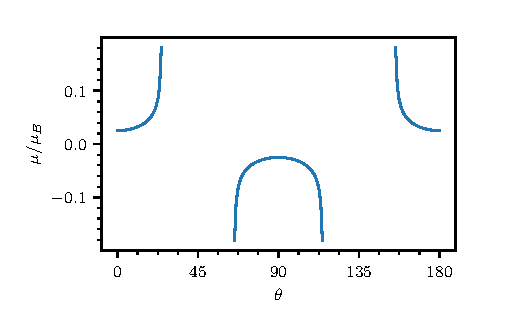
\includegraphics{non-polar-plot-sign}
		\caption{For angles $\theta$ of the spin demon in the altermagnetic spin-split plane, its magnetic moment. The equivalent of the colorscale in \cref{fig:magnetic-moment} in the main text. \label{fig:magnetic-moment-SM}}
	\end{figure}
	
	
	\subsection{Conventional plasmon}
	The conventional plasmon is also present, but lives outside of the electron-hole continuum of either spin species. It can therefore be found by taking the dynamical long-wavelength limit,\footnote{This corresponds to expanding in small $v_Fq/\omega$ along the $\omega$ axis. } such that $\chi_{\sigma}^{(0)}=\frac{n_0 \eta_\sigma^2 q_\sigma^2}{\mdos \omega^2}$ \cite{giulianiQuantumTheoryElectron2005}. This gives the conventional solutions to $\Ree[\epsilon(\bm q,\omega)]=0$ as 
	\begin{equation}
		\omega^2 = \frac{n_0 e^2}{\mdos\epsilon_0} + O(\bar q^2),
	\end{equation}
	which is a gapped plasmon, with a gap $\hbar\sqrt{\frac{n_0 e^2}{\mdos\epsilon_0}}\approx 4\epsilon_F$. Here, $n_0\equiv\sum_\sigma n_\sigma=\frac{4}{3}N_0\epsilon_F$. 
	
	\section{Spin demon for larger wave vectors}
	In the main text, we consider the limit $q/\kF\ll1$, for which the spin demon dispersion is approximately linear in $q$. Here we investigate the dispersion and damping of the spin demon for larger wave vectors, and show the spin-spin response function $\Imm[\chi_{S_zS_z}(\bm q,\omega)]$ for a larger range of wave vector $q$ in \cref{fig:larger-q}. We first observe that for small wave vectors $q/\kF$, there is a well-defined spin demon. At approximately $q/\kF\approx 0.5$, the spin demon becomes overdamped, and ceases to be well defined. These results suggest that over a large range of wave vectors, the spin demon is well defined and can be measured.
	
	\begin{figure}
		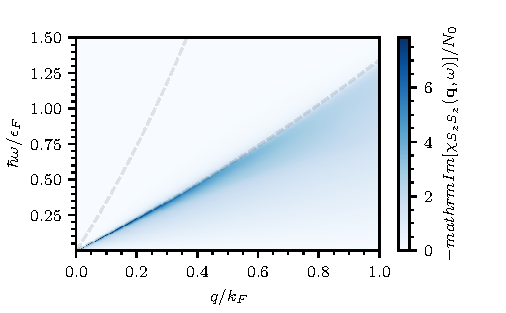
\includegraphics{SzSz_3D_large_range}
		\caption{The spin-spin response function $\Imm[\chi_{S_zS_z}(\bm q,\omega)]$ for $\bm q =q\hat{\bm x}$, for a larger range of wave vector $q$. At $q/\kF\approx 0.5$ the spin demon becomes overdamped, and ceases to be well defined. The dashed lines indicate the edges of the spin-up and spin-down particle-hole continuum, $\omega_{+\sigma}$. }
		\label{fig:larger-q}
	\end{figure}
	
	\section{Two dimensions}
	We now consider a two-dimensional $d$-wave altermagnet, with the dispersion
	\begin{align}
		\epsilon_{\bm k}^\sigma &= \frac{\hbar k^2}{2m_0} + \sigma \frac{\hbar k_x^2}{2m_*} - \sigma \frac{\hbar k_y^2}{2m_*} \\
		&=\frac{\hbar k_x^2}{2m_x^\sigma}+ \frac{\hbar k_y^2}{2m_y^\sigma}
	\end{align}
	Again, within this orientation, the altermagnetic spin splitting is maximal along the $x$- and $y$-directions. Note that $m_{x,y}^\sigma$ are defined in \cref{eq:mx,eq:my}.
	%	 We choose the Fermi level $\epsilon_F^\mathrm{2D} = ({(m_*^2 - m_0^2)/m_*^2})^{1/6}\epsilon_F^\mathrm{3D}$ to reproduce the same spin splitting at the Fermi level. Here, $({(m_*^2 - m_0^2)/m_*^2})^{1/6}\approx\twoDratio$.
	
	In two dimensions, the Lindhard function at zero temperature is given by \cite{ahnAnisotropicFermionicQuasiparticles2021}
	\begin{multline}
		-\frac{\Ree[\chi_\sigma^{(0)} (\bm q,\omega) ]}{N_0 }= 1 + \frac{1}{\eta_\sigma \bar q} \bigg[\sign(\nu_{-\sigma}) \Theta(\nu_{-\sigma}^2-1)\sqrt{\nu_{-\sigma}^2-1}\\+\sign(\nu_{+\sigma}) \Theta(\nu_{+\sigma}^2-1)\sqrt{\nu_{+\sigma}^2-1}\bigg]
	\end{multline}
	and 
	\begin{multline}
		-\frac{\Imm[\chi_\sigma^{(0)} (\bm q,\omega) ]}{ N_0}=\Theta(1-\nu_{-\sigma}^2)\sqrt{1-\nu_{-\sigma}^2}\\-\Theta(1-\nu_{+\sigma}^2)\sqrt{1-\nu_{+\sigma}^2},
	\end{multline}
	where $\eta_\sigma$ is defined in \cref{eq:sigma}, but with
	$\mdos\equiv \sqrt{m_xm_y}$. The definition of $\nu_{\pm\sigma}$ is unchanged. At $m_x^\sigma=m_y^\sigma$ this reduces to the well-known isotropic result \cite{giulianiQuantumTheoryElectron2005}. Finally, $N_0=\mdos/2\pi\hbar^2$ is the density of states per spin.
	Additionally, we now have that $v_q=e^2/(2\pi\epsilon_0 q)$.
	
	
	
	%	As was pointed out by \textcite{agarwalLonglivedSpinPlasmons2014}, within a pseudo-gap formed by the spin-up and spin-down electron-hole continuum there exist a spin plasmon. Specifically, the pseudo gap is given by 
	%	\begin{equation}
		%		\begin{cases}
			%			\omega_{+\downarrow}<\omega<\omega_{+\uparrow} \quad &\mathrm{if}\quad \omega_{+\downarrow}<\omega_{+\uparrow} \\ 
			%			\omega_{+\uparrow}<\omega<\omega_{+\downarrow} \quad &\mathrm{if}\quad \omega_{+\downarrow}>\omega_{+\uparrow}
			%		\end{cases}
		%	\end{equation}
	%	where $\omega_{+\sigma}=\tilde q_\sigma^2/2\mdos+v_F\tilde q_\sigma$ is the upper boundary of the electron-hole continuum with spin $\sigma$. Here we stress that $\tilde q_\sigma$ incorporates the four-fold $d$-wave altermagnetic symmetry, such that for $\bm q\parallel \bm x$ we have that $\omega_{+\downarrow}<\omega_{+\uparrow}$, whereas for $\bm q\parallel\bm y$ we have $\omega_{+\downarrow}>\omega_{+\uparrow}$. 
	As before, we first take $\bm q\parallel\xx$. Then we have that $\Ree[\chi_{\uparrow}^{(0)}(\bm q,\omega)]=-N_0$,\footnote{In contrast to the three-dimensional case, in two dimensions the particle-hole continuum is constant for $\omega<\omega_{+}$ and this result is thus exact.}  and 
	\begin{equation}
		-\chi_\downarrow^{(0)} (\bm q,\omega) / N_0 = 1 + \frac{\kF}{\eta_\downarrow q} \left[\sqrt{\nu_{-\downarrow}^2-1}-\sqrt{\nu_{+\downarrow}^2-1}\right].
	\end{equation} 
	In contrast to the three-dimensional case, we can now find exact solutions to $\Ree[\epsilon(\bm q,\omega)]=0$ as \cite{agarwalLonglivedSpinPlasmons2014}
	\begin{equation}
		\omega = \eta_{\downarrow} qv_F \sqrt{\frac{1}{1-V_q^2} + \frac{(\eta_\downarrow q)^2}{4\kF^2V_q^2}},
	\end{equation}
	where $V_q \equiv \frac{v_qN_0}{1+2v_qN_0}$.
	The solutions for $\bm q\parallel \yy $  follow analogously, by changing $\downarrow$ to $\uparrow$. 
	
	Taking the limit of $q\rightarrow0$, we have that $V_q=1/2$ and thus
	\begin{equation}
		\omega_d=\frac{2}{\sqrt{3}} v_F \eta_\downarrow q. \label{eq:ws-2D}
	\end{equation}
	Secondly, we require that $\omega_{d}<\omega_{+\downarrow}$, which implies that (up to order $O(\bar q^2)$),
	\begin{equation}
		\frac{\eta_{\uparrow}}{\eta_{\downarrow}} < \frac{\sqrt{3}}{2}, \label{eq:stability-2D}
	\end{equation}
	which gives the critical angle
	\begin{equation}
		\cos2\theta_c =  \frac{m_*}{7m_0},
	\end{equation}
	which for the parameters used in the main text is $\theta_c=\criticalangle$.
	
	We compare this result in \cref{fig:compare2D} with the numerical results, by overlaying the resulting dispersion with $\Imm[\chi_{S_zS_z}]$. We observe that close to the $x,y$-axis, the analytical spin demon dispersion closely reproduces the numerical results. For angles away from the $x,y$-axis, this is no longer the case, and the spin demon frequency is overestimated. In addition, the numerical results indicate that the spin demon persists for angles close to $\theta=\SI{45}{\degree}$, whilst our analysis predicts a critical angle of $\criticalangle$. 
	\begin{figure}
		\includegraphics{2D_polar-plot-chiSzSz-with-vs}
		\caption{In two dimensions, $\Imm[\chi_{S_zS_z}]$ compared against the spin demon dispersion found in \cref{eq:ws-2D}. We only show the spin demon solution where the condition in \cref{eq:stability-2D} is fulfilled.  \label{fig:compare2D} }
	\end{figure}
	
	
	
	\subsection{Damping}
	We determine the damping of the spin demon analogous to the three-dimensional altermagnet (\cref{sec:damping}). Again, the imaginary part of the dielectric function is only governed by the majority-spin electrons, such that 
	\begin{align}
		\Imm[\epsilon] &= v_q N_0 \frac{\kF}{\eta_\uparrow q} \left[\sqrt{1-\nu_{-\uparrow}^2}-\sqrt{1-\nu_{+\uparrow}^2}\right] \\
		&\overset{\omega\rightarrow\omega_{d}}{=}N_0v_q\frac{2\eta_\downarrow}{\sqrt{4\eta_\downarrow^2-3\eta_\uparrow^2}}+ O(\bar q^2)
	\end{align}
	where in the second line we have inserted the spin demon solution and expanded up to second order in $\bar q$.
	The derivative of the dielectric function is given by
	\begin{align}
		\partial_\omega \Ree[\epsilon] = -&\frac{v_q N_0 \kF}{\eta_\downarrow q} \partial_\omega \left(\sqrt{\nu_{-\downarrow}^2-1}-\sqrt{\nu_{+\downarrow}^2-1}\right) \\ 
		\overset{\omega\rightarrow\omega_{d}}{=}&N_0\frac{3\sqrt{3} v_q}{v_F q\eta_\downarrow} + O(\bar q^0)\\
		=&N_0\frac{6v_q}{\omega_{d}}+ O(\bar q^0)
	\end{align}
	where we have again inserted the spin demon solution and expanded up to zeroth order in $\bar q$.
	The damping rate is now given by
	\begin{equation}
		\gamma = \omega_{d}\frac{\eta_\downarrow}{3\sqrt{4\eta_\downarrow^2-3\eta_\uparrow^2}}
	\end{equation}
	and the quality factor thus is
	\begin{equation}
		Q = \frac{3\sqrt{4\eta_\downarrow^2-3\eta_\uparrow^2}}{\eta_\downarrow}.
	\end{equation}
	
	\subsection{Magnetic moment and out-of-phase oscillations}
	In addition, we can find the corresponding amplitudes of the spin demon by solving the eigenvalue problem 
	\begin{equation}
		\begin{pmatrix}
			\Re[\chi_{\uparrow}^{(0)}(\omega)]^{-1}-v_q & -v_q \\
			-v_q & \Re[\chi_{\downarrow}^{(0)}(\omega)]^{-1}-v_q
		\end{pmatrix}\begin{pmatrix}
			\psi_\uparrow \\ \psi_\downarrow
		\end{pmatrix} =0
	\end{equation}
	which can again be solved by noting that for $\bm q\parallel\xx$, $\Ree[\chi_\uparrow]=-N_0$, to find
	%	\begin{equation}
		%		\frac{\psi_\uparrow}{\psi_\downarrow} = 
		%		-\begin{cases}
			%			\frac{v_q N_0}{1+v_qN_0} \quad &\mathrm{if}\quad \omega_{+\downarrow}<\omega_{+\uparrow}  \\
			%			\frac{1+v_qN_0}{v_q N_0} \quad &\mathrm{if}\quad \omega_{+\downarrow}>\omega_{+\uparrow}
			%		\end{cases}
		%	\end{equation}
	\begin{equation}
		\frac{\psi_\uparrow}{\psi_\downarrow} = 
		-
		\frac{v_q N_0}{1+v_qN_0} = -1 + O(\bar q).
	\end{equation}
	Thus, at finite wavelength the spin demon correspond to  out of phase oscillations of the spin up and down modes, which are dominated by the spin-down component for $\bm q\parallel \xx$.
	
	To determine the magnetic moment of the spin demon, we again introduce a small magnetic field along the quantization axis, such that
	\begin{equation}
		\epsilon_{\bm k}^\sigma = \frac{\hbar k^2}{2m_0} + \sigma \frac{\hbar k_x^2}{2m_*} - \sigma \frac{\hbar k_y^2}{2m_*} + \sigma g_e\mu_B B.
	\end{equation} 
	This results in a shift of the Fermi wave vector, $\kF^\sigma\rightarrow \kF\sqrt{1-\sigma g_e\mu_B B / \epsilon_F}$. We can  directly write down the resulting dispersion relation from \cref{eq:ws-2D} as
	\begin{equation}
		\omega_{d}=\frac{2}{\sqrt{3}} v_F \eta_\downarrow q \sqrt{1+g\mu_B B / \epsilon_F}.
	\end{equation}
	The resulting magnetic moment, as defined in \cref{eq:magnetic-moment} is 
	\begin{equation}
		\mu_p = \frac{2}{\sqrt{3}} v_F \eta_\downarrow q \frac{g\mu_B}{\epsilon_F} + O((g\mu_B B / \epsilon_F)^2),
	\end{equation}
	where we remind the reader that this result only holds for $\bm q\parallel \xx$, and for $\bm q\parallel \yy$ we obtain the opposite magnetic moment, since the roles of the minority and majority spin species is reversed. We show the resulting magnetic moment in \cref{fig:2D-magnetic-moment}, where we observe the same features as in the three-dimensional case: the magnetic moment follows the $d$-wave symmetry, changing sign in the four different quadrants of the plane. Additionally, the magnetic moment has a value of $|\mu_p|\approx 0.1\mu_B$ for $\bm q\parallel\xx$ and $\bm q\parallel\yy$, and grows to $|\mu_p|\approx 0.35\mu_B$ close to the diagonals---but we remind the reader that the quality factor drops off sharply, and the spin demon will thus be significantly damped. These are comparable in magnitude to the three-dimensional altermagnet.
	
	\begin{figure}
		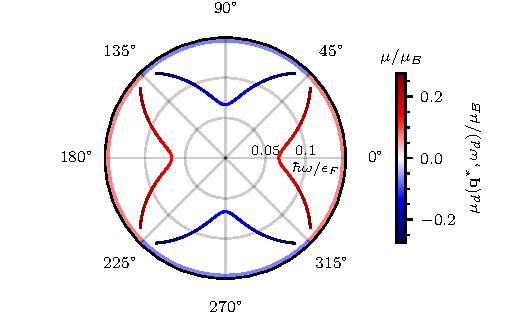
\includegraphics{2D-polar-plot-sign}
		\caption{In two dimensions, the frequency and magnetic moment (color scale) of the spin demon as a function of angle $\theta$. The magnetic moment has a value of $|\mu_p|\approx 0.1\mu_B$ for $\bm q\parallel\xx$ and $\bm q\parallel\yy$ \label{fig:2D-magnetic-moment}}
	\end{figure}
	
	\subsection{Conventional plasmon}
	If we instead take the dynamical long-wavelength limit, such that $\chi_{\sigma}^{(0)}=\frac{n_0 \tilde q_\sigma^2}{\mdos \omega^2}$, we obtain the conventional plasmon with
	\begin{equation}
		\omega^2 = \frac{2\pi e^2n_0}{\epsilon m_0} q + O(\bar q^2),
	\end{equation}
	where $n_0=\sum_\sigma n_\sigma=2N_0\epsilon_Fq$ is the total electron density.
	
	
	
	\section{$g$-wave altermagnet}
	Here, we show that the splitting of the particle-hole continua in a higher order altermagnet is not sufficient for the emergence of a spin demon. Specifically, we consider a three-dimensional $g$-wave altermagnet, where the low-energy electron dispersion of spin $\sigma$ can be written as \cite{smejkalConventionalFerromagnetismAntiferromagnetism2022}
	\begin{align}
		\epsilon_{\bm k}^\sigma &= \frac{\hbar^2 k^2}{2m_0} + \sigma \Delta  k_xk_z\left(k_x^2-3k_y^2\right).
	\end{align}
	Here $\Delta$ is the strength of the splitting. In contrast to the $d$-wave altermagnet, the spin splitting parameter $\Delta$ cannot have an arbitrary strength, due to its higher momentum power. I.e., for strong $\Delta$ the curvature of the bands is negative. Specifically, at the Fermi level, along one of the maximum-splitting directions [such as $\bm k = k\  (\sqrt{3}/2,0,1/2)$], we have that 
	\begin{equation}
		\kF^\sigma = \frac{2}{3^{3/4}} \sqrt{\frac{\sqrt{\hbar^4+ 3\sqrt{3}\sigma E_Fm_0^2 \Delta  }-\hbar^2}{m_0 \Delta} } \label{eq:kF-g-wave}
		%		\sqrt{\frac{\hbar^2/2m - \sqrt{(\hbar^2/2m)^2 -3\sqrt{3}/4\sigma\Delta E_F }}{3\sqrt{3}/8 \Delta}}iu
	\end{equation}
	and we find that the group velocity at the Fermi level is positive for both spin $\sigma$ if
	\begin{equation}
		\Delta < \frac{\hbar^2}{3\sqrt{3}E_F m_0 }. \label{eq:delta-condition}
	\end{equation}
	
	We thus have a constraint on the spin splitting $\Delta$, which also constraints the separation of the spin-polarized particle-hole continua.  
	
	
	
	%	Specifically, at zero temperature, the particle-hole continuum is given as the region where 
	%	\begin{multline}
		%		\Imm[\chi_\sigma] =\\ -\frac{\pi}{N}\sum_{\bm k} \sum_{\bm k}\left[ \Theta(\epsilon_{\bm k}^\sigma-E_F) - \Theta(\epsilon_{\bm k+\bm q}^\sigma-E_F) \right] \delta(\hbar\omega+\epsilon_{\bm k}^\sigma-\epsilon_{\bm k+\bm q}^\sigma)
		%	\end{multline}
	%	is non-zero \cite{giulianiQuantumTheoryElectron2005}. One can now directly read off the upper edge of the spin-polarized particle-hole continuum for  $q\ll \hat{\bm q}\cdot \bm \kF$ as
	%	\begin{equation}
		%		\omega_{+\sigma}=\bm v_{F\sigma} \cdot \bm q + O\left(\left(\frac{q}{\hat{\bm q}\cdot \bm \kF}\right)^2\right).
		%	\end{equation}
	%	We stress however that this result only gives the upper edge of the continuum, and does not give us information about the internal structure of the continuum. The internal structure of the continuum will be more involved, owing to the non-isotropic nature of the Fermi surfaces in a $g$-wave altermagnet.
	%	%	and thus we have that for $\bm q$ along one of the maximum-splitting directions the upper edge of the spin-polarized particle-hole continuum is 
	%%	\begin{equation}
		%%		\omega_{+\sigma} = \left(\frac{\hbar}{m_0} k_{F\sigma} + \sigma \frac{3\sqrt{3}}{4}\Delta k_{F\sigma}^3 \right) q,
		%%	\end{equation}
	%%	where $k_{F\sigma}$ is the spin-dependent Fermi wave vector along one of the maximum-splitting direction, as given by \cref{eq:kF-g-wave}. 
	%	
	%	We now first continue to work out the possible maximal separation of the spin-polarized particle-hole continua.
	%	We choose $\Delta = \frac{\hbar^2}{3\sqrt{3}E_F m_0 }$, order to obtain a maximum spin splitting, while retaining a positive curvature at the Fermi level.\footnote{Formally, we obtain here a zero group velocity.} After some manipulation, we can write the maximally possible separation of the spin-polarized particle-hole continua as 
	%	\begin{equation}
		%		\omega_{+\uparrow} - \omega_{+\downarrow} \overset{\Delta=\hbar^2/3\sqrt{3}E_F m_0 }{=} \frac{1}{\hbar}\sqrt{\frac{\hbar^2 E_F}{2m_0}}q.
		%	\end{equation}
	%%	This result indicates that even with $\Delta$ chosen such that there is a maximal spin splitting, the seperation between the spin-polarized particle-hole continua grows as $\propto \sqrt{E_F/m_0}$. 
	%
	%	
	%	
	%	In contrast, for a $d$-wave altermagnet, the separation of the spin-polarized particle-hole continua along a maximal splitting direction is given by [choosing $\bm q = q \hat{\bm x}$ here]
	%	\begin{equation}
		%		\omega_{+\uparrow} - \omega_{+\downarrow} = \sqrt{2E_Fm_0m_*}\left(\sqrt{\frac{1}{m_*+m_0}}-\sqrt{\frac{1}{m_*-m_0}}\right)q.
		%	\end{equation}
	%	In a $d$-wave altermagnet, $\sqrt{\frac{1}{m_*+m_0}}-\sqrt{\frac{1}{m_*-m_0}}$ can be made arbitarily large, since the spin splitting occurs already in the quadratic part of the dispersion. There is thus no such requirement as \cref{eq:delta-condition}, and one can realize the large separation of the particle-hole continua as demonstrated in the main text.
	
	
	We now numerically calculate $\chi_{\sigma}(\bm q,\omega)$ for a $g$-wave altermagnet. We show $\chi_{\sigma}(\bm q,\omega)$ in \cref{fig:g-wave}, together with the complex longitudinal dielectric function, $\epsilon(\bm q,\omega)$, along a maximual-splitting direction $\bm q = q\, \left(\sqrt{3}/2,0,1/2\right)$. We have chosen $q=0.05\kF^0$ and $\Delta ={\hbar^2}/{3\sqrt{3}E_F m_0 }$, in order to obtain maximal separation of the spin-polarized particle-hole continua. Finally, we set $e^2/\epsilon = 80 E_F/\kF^0$. We have defined $\kF^0\equiv \sqrt{2m_0E_F}/\hbar$ for convenience. 
	
	We observe that the particle-hole continua are separated, similar to the $d$-wave altermagnet, except that the separation is much smaller (compare with \cref{fig:alongx} in the main text). Importantly, it is not possible to further increase the splitting by increasing $\Delta$, since this would violate the condition in \cref{eq:delta-condition}. We therefore conclude that the long-wavelength dispersion of a $g$-wave altermagnet is ill-suited for the emergence of a spin demon.
	
	\begin{figure}
		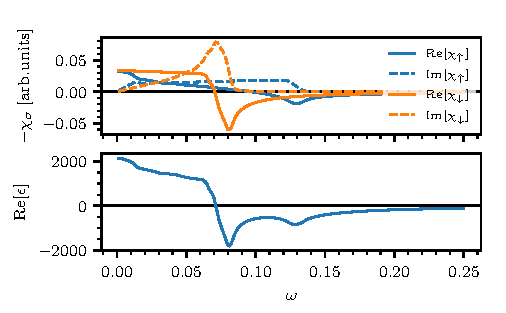
\includegraphics{g-wave}
		\caption{For a bulk $g$-wave altermagnet, the real and imaginary part of $\chi_{\sigma}$, and the real part of the complex longitudinal dielectric function.}
		\label{fig:g-wave}
	\end{figure}
	
	\bibliography{spin-plasmons}
\end{document}
